% !TeX root = surprises.tex

\chapter{El problema de Langford}\label{c.langford}

%%%%%%%%%%%%%%%%%%%%%%%%%%%%%%%%%%%%%%%%%%%%%%%%%%%%%%%%%%%%%%%

C. Dudley Langford se dio cuenta de que su hijo había ordenado los bloques de colores como se muestra en la Fig.~\ref{f.langford}.
Hay un bloque entre los bloques rojos, dos bloques entre los bloques azules y tres bloques entre los bloques verdes. 

\begin{figure}[ht]
\begin{center}
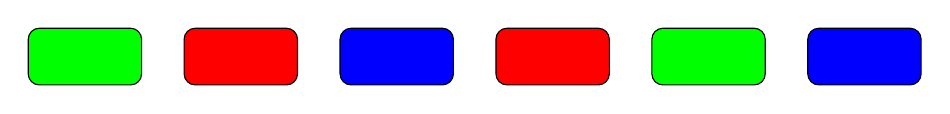
\begin{tikzpicture}[scale=.9]
\draw[rounded corners,fill=green] (0,0)  
  rectangle +(1.6cm,.8cm);
\draw[rounded corners,fill=red]   (2.2,0)
  rectangle +(1.6cm,.8cm);
\draw[rounded corners,fill=blue]  (4.4,0)
  rectangle +(1.6cm,.8cm);
\draw[rounded corners,fill=red]   (6.6,0)
  rectangle +(1.6cm,.8cm);
\draw[rounded corners,fill=green] (8.8,0)
  rectangle +(1.6cm,.8cm);
\draw[rounded corners,fill=blue]  (11,0)
  rectangle +(1.6cm,.8cm);
\end{tikzpicture}
\end{center}
\caption{Disposición de los bloques para el problema de Langford}\label{f.langford}
\end{figure}

\begin{definition}[Problema de Langford $L(n)$] Dado el multiconjunto \footnote{Un \emph{multiconjunto} o \emph{bolsa} es como un conjunto excepto que puede haber más de una ocurrencia de un elemento.} de números enteros positivos:
\[
\{1,1,2,2,3,3,\ldots,n,n\}\,,
\]
¿pueden ordenarse en una secuencia tal que para $1\leq i \leq n$ haya $i$ números entre las dos ocurrencias de $i$?
\end{definition}

Figura~\ref{f.langford} muestra que 312132 es una solución para $L(3)$.

Sección~\ref{s.langford-covering} replantea el problema de Langford utilizando un formalismo matemático que facilita la resolución del problema. La sección~\ref{s.langford-theorem} caracteriza los valores de $n$ para los que $L(n)$ es resoluble y presenta dos pruebas del teorema. La primera, relativamente sencilla, utiliza la técnica del doble recuento: contar el mismo valor de dos formas distintas e igualar las fórmulas resultantes. La segunda prueba es una inducción inteligente, pero la "contabilidad" que implica requiere una cuidadosa atención a los detalles. Sección~\ref{s.langford-four} resuelve la solución para $L(4)$.

\section{El problema de Langford como un problema de cobertura}\label{s.langford-covering}

El problema de Langford se puede plantear utilizando una matriz. Para $L(3)$ hay seis columnas, una para cada posición en la que se pueden colocar los seis números. Hay una fila para cada posible colocación de uno de los números, es decir, las dos ocurrencias de $k$ deben tener $k$ números entre ellos. Hay cuatro colocaciones posibles de $1$, tres de $2$ y dos de $3$:

\begin{center}
\addtolength{\tabcolsep}{4pt}
\begin{tabular}{|c||c|c|c|c|c|c|}
\hline
&1&2&3&4&5&6\\\hline\hline
1&1&&1&&&\\\hline
2&&1&&1&&\\\hline
3&&&1&&1&\\\hline
4&&&&1&&1\\\hline
5&2&&&2&&\\\hline
6&&2&&&2&\\\hline
7&&&2&&&2\\\hline
8&3&&&&3&\\\hline
9&&3&&&&3\\\hline
\end{tabular}
\end{center}
Para resolver el problema tenemos que seleccionar una fila para los $1$ de la secuencia, una fila para los $2$ y una fila para los $3$, de tal forma que si apilamos estas filas unas sobre otras, ninguna columna contenga más de un número.

No es necesario considerar la fila 9 debido a la simetría: empezar por la fila 9 sólo da la inversa de la secuencia obtenida al empezar por la fila 8.

La fila 8 es la única que contiene $3$'s por lo que debe ser elegida y la secuencia es 3\textvisiblespace \textvisiblespace \textvisiblespace 3\textvisiblespace. Ya no se puede utilizar ninguna fila con números en las columnas 1 y 5, porque sólo se puede colocar un número en cada posición. Denotemos las filas permitidas y prohibidas por:
\[\not\! 1,2,\not\! 3,4,\not\! 5, \not\! 6, 7, 8\,.\]

La fila 7 es la única fila restante que contiene $2$, por lo que debe elegirse y la secuencia es 3\textvisiblespace 2\textvisiblespace 3{}2. La eliminación de las filas que ya no se puede utilizar da:
\[\not\! 1,2,\not\! 3,\not\! 4,\not\! 5, \not\! 6, 7, 8\,.\]

Eligiendo la única fila que queda, la fila 2, se obtiene la solución 3{}1{}2{}1{}3{}2:
\begin{center}
\addtolength{\tabcolsep}{4pt}
\begin{tabular}{|c||c|c|c|c|c|c|}
\hline
&1&2&3&4&5&6\\\hline\hline
2&&1&&1&&\\\hline
7&&&2&&&2\\\hline
8&3&&&&3&\\\hline
\end{tabular}
\end{center}
El análisis ha demostrado que ésta es la única solución, salvo la solución simétrica obtenida empezando por la fila 9.

\section{¿Para qué valores de $N$ se puede resolver el problema de Langford?}\label{s.langford-theorem}

\begin{theorem} \label{thm.langford}
$L(n)$ tiene solución si y sólo si $n=4k$ o $n=4k+3$.
\end{theorem}\index{Langford's problem!solvability, conditions for}

Demostramos el sentido directo del teorema. La prueba~1 muestra que si $L(n)$ tiene solución entonces $n=4k$ o $n=4k+3$. La prueba~2 muestra el contrapositivo: si $n=4k+1$ o $n=4k+2$ entonces $L(n)$ no tiene solución.

\begin{proof}
\mbox{}\\
(1)
Si la primera ocurrencia del número $k$ está en la posición $i_k$, la segunda ocurrencia está en la posición $i_k+k+1$. Por ejemplo, en 3{}1{}2{}1{}3{}2, la solución para $L(3)$, eligiendo $k=2$ se obtiene $i_k=3$ y $i_k+k+1=3+2+1=6$.

$S_n$, la suma de las posiciones de todos los números, es:
\begin{eqnarray*}
S_n&=&\sum_{k=1}^{n}i_k+\sum_{k=1}^{n}(i_k+k+1)\\
& =& 2\sum_{k=1}^{n}i_k+\sum_{k=1}^{n}(k+1)\\
&=& 2\sum_{k=1}^{n}i_k+\frac{n(n+3)}{2}\,.
\end{eqnarray*}
Pero $S_n$ es simplemente $1+2+3+\cdots+2n$, así que:
\[
S_n=\sum_{k=1}^{2n}k = \frac{2n(2n+1)}{2}\,.
\]
Igualando las dos fórmulas para $S_n$ se obtiene:
\begin{eqnarray*}
2\sum_{k=1}^{n}i_k+\frac{n(n+3)}{2} &=& \frac{2n(2n+1)}{2}\\
\sum_{k=1}^{n}i_k &=& \frac{1}{2}\left(\frac{2n(2n+1)}{2} - \frac{n(n+3)}{2}\right) \\
&=& \frac{3n^2-n}{4}\,.
\end{eqnarray*}

El lado izquierdo es un entero ya que es la suma de enteros (las posiciones), por lo que el lado derecho también debe ser un entero. ¿Cuándo es $3n^3-n$ divisible por $4$? Al factorizar $3n^2-n$ se obtiene $n(3n-1)$.

Si $n$ es múltiplo de $4$, el producto es divisible por $4$.

¿Cuándo $3n-1$ es divisible por $4$? Cualquier número entero $n$ se puede expresar como $n=4i+j$ para $j=0,1,2,3$. Si $3n-1$ es divisible por $4$, entonces también lo es $3(4i+j)-1 = 12i+3j-1$. $12i$ es divisible por $4$. Para $j=\{0,1,2,3\}$, $3j-1=\{-1,2,5,8\}$ es divisible por $4$ si y sólo si $j=3$, es decir, $n=4i+3$.
\end{proof}

Para introducir la idea de la segunda prueba, considere cómo podría ser una solución para $n=4$. En las tablas siguientes las posiciones de las apariciones de 4 son 1 y 6, y las posiciones de las apariciones de 2 son 5 y 8. En ambos casos, una posición es impar y la otra par. En ambos casos, una posición es impar y la otra par. 
\[
\addtolength{\arraycolsep}{4pt}
\begin{array}{|c|c|c|c|c|c|c|c|}
\hline
1&2&3&4&5&6&7&8\\
\hline\hline
4&1&3&1&2&4&3&2\\\hline
*&&&&&*&&\\\hline
\end{array}
\hspace{3em}
\begin{array}{|c|c|c|c|c|c|c|c|}
\hline
1&2&3&4&5&6&7&8\\
\hline\hline
4&1&3&1&2&4&3&2\\\hline
&&&&*&&&*\\\hline
\end{array}
\]
Sea $k=2m$ un número \emph{par}. Si $i$ es la posición de la primera ocurrencia de $k$, entonces la posición de la segunda ocurrencia es $i+k+1$.
La suma de las posiciones es:
\[
i+(i+k+1)=2i+2m+1=2(i+m)+1\,,
\]
que es un número impar. Para que la suma de dos números sea impar, uno debe ser impar y el otro par.

Comprobemos ahora las posiciones de los números impares. Las posiciones de las apariciones de 1 son 2 y 4, ambos números pares, y las posiciones de las apariciones de 3 son 3 y 7, ambos números impares.
\[
\addtolength{\arraycolsep}{4pt}
\begin{array}{|c|c|c|c|c|c|c|c|}
\hline
1&2&3&4&5&6&7&8\\
\hline\hline
4&1&3&1&2&4&3&2\\\hline
&*&&*&&&&\\\hline
\end{array}
\hspace{3em}
\begin{array}{|c|c|c|c|c|c|c|c|}
\hline
1&2&3&4&5&6&7&8\\
\hline\hline
4&1&3&1&2&4&3&2\\\hline
&&*&&&&*&\\\hline
\end{array}
\]
Sea $k=2m+1$ un número \emph{impar}. La suma de las posiciones es:
\[
i+(i+k+1)=2i+2m+1+1=2(i+m+1)\,,
\]
que es un número par. Para que la suma de dos números sea par, ambos deben ser impares o ambos pares.

Las posiciones $1,2,\ldots,2n-1,2n$ contienen igual número de posiciones pares e impares. Las dos apariciones de un número en una fila ``cubren'' dos posiciones. Cuando el conjunto de filas cubre todas las posiciones, deben cubrir igual número de posiciones pares e impares. Definimos la \emph{paridad} de un conjunto de filas como la diferencia entre el número de posiciones pares e impares cubiertas. Inicialmente, la paridad es cero, y si el problema tiene una solución, el conjunto de filas en la solución también tiene paridad cero.

Cuando se colocan dos ocurrencias de un número par, cubren una posición par y una impar, por lo que la paridad sigue siendo la misma:
\[
\addtolength{\arraycolsep}{4pt}
\begin{array}{|c|c|c|c|c|c|c|c|}
\hline
1&2&3&4&5&6&7&8\\
\hline\hline
4&1&3&1&2&4&3&2\\\hline
-1&&&&&+1&&\\\hline
\end{array}
\hspace{3em}
\begin{array}{|c|c|c|c|c|c|c|c|}
\hline
1&2&3&4&5&6&7&8\\
\hline\hline
4&1&3&1&2&4&3&2\\\hline
&&&&-1&&&+1\\\hline
\end{array}
\]
Cuando se colocan dos ocurrencias de un número impar, la paridad se convierte en $+2$ o $-2$, por lo que debemos ser capaces de asociar este par con un par de ocurrencias de \emph{otro} número impar que se coloquen en posiciones que equilibren la paridad:
\[
\addtolength{\arraycolsep}{4pt}
\begin{array}{|c|c|c|c|c|c|c|c|}
\hline
1&2&3&4&5&6&7&8\\
\hline\hline
4&1&3&1&2&4&3&2\\\hline
&+1&&+1&&&&\\\hline
\end{array}
\hspace{3em}
\begin{array}{|c|c|c|c|c|c|c|c|}
\hline
1&2&3&4&5&6&7&8\\
\hline\hline
4&1&3&1&2&4&3&2\\\hline
&&-1&&&&-1&\\\hline
\end{array}
\]
Hemos demostrado que puede haber una solución al problema de Langford si y sólo si ¡hay un número par de números impares en $\{1,\ldots,n\}$!
El teorema afirma que si esto es cierto entonces o $n=4k$ o $n=4k-1$, y si no entonces o $n=4k-2$ o $4k-3$.

\begin{proof}
\mbox{}\\
(2)
La prueba es por inducción.
Hay cuatro casos base:
\begin{itemize}
\item $n=4k-3=1$. En $\{1\}$ hay un número impar de números impares y no hay solución.
\item $n=4k-2=2$. En $\{1,2\}$ hay un número impar de números impares y no hay solución.
\item $n=4k-1=3$. En $\{1,2,3\}$ hay un número par de números impares y hemos visto que hay solución.
\item $n=4k-0$. En $\{1,2,3,4\}$ hay un número par de números impares y Sect.~\ref{s.langford-four} da una solución.
\end{itemize}

La hipótesis inductiva es que el teorema es cierto para $\{1,\ldots,4k-j\}$, $k\ge 1$, $0\leq j\leq 3$, y demostraremos que es cierto para $n=4(k+1)-j$.

\begin{itemize}
\item Añadir $4k+1=4(k+1)-3$ a $\{1,\ldots,4k\}$. Por la hipótesis inductiva para $4k=4k-0$ hay un número par de impares. $4(k+1)-3$ es impar por lo que ahora hay un número impar de números impares y no hay solución.
\item Añadir $4k+2=4(k+1)-2$ a $\{1,\ldots,4k+1\}$. Por la hipótesis inductiva para $4k+1=4(k+1)-3$ hay un número impar de números impares. $4(k+1)-2$ es par por lo que sigue habiendo un número impar de números impares y no hay solución.
\item Añadir $4k+3=4(k+1)-1$ a $\{1,\ldots,4k+2\}$. Por la hipótesis inductiva para $4k+2=4(k+1)-2$ hay un número impar de números impares. $4(k+1)-1$ es impar por lo que hay un número par de números impares y es probable que exista una solución.
\item Añadir $4k+4=4(k+1)-0$ a $\{1,2,\ldots,4k+3\}$. Por la hipótesis inductiva para $4k+3=4(k+1)-1$ hay un número par de impares. $4(k+1)-0$ es par por lo que hay un número par de números impares y es probable que exista una solución.
\end{itemize}
\end{proof}

%%%%%%%%%%%% Solution for L(4) %%%%%%%%%%%%%%%%%%



\section{Solución para $L(4)$}\label{s.langford-four}

\index{Langford's problem!solution of $L(4)$}
Aquí está la matriz para $L(4)$. Intenta encontrar la solución tú mismo.
\begin{center}
\addtolength{\tabcolsep}{4pt}
\begin{tabular}{|c||c|c|c|c|c|c|c|c|}
\hline
&1&2&3&4&5&6&7&8\\\hline\hline
1&1&&1&&&&&\\\hline
2&&1&&1&&&&\\\hline
3&&&1&&1&&&\\\hline
4&&&&1&&1&&\\\hline
5&&&&&1&&1&\\\hline
6&&&&&&1&&1\\\hline
7&2&&&2&&&&\\\hline
8&&2&&&2&&&\\\hline
9&&&2&&&2&&\\\hline
10&&&&2&&&2&\\\hline
11&&&&&2&&&2\\\hline
12&3&&&&3&&&\\\hline
13&&3&&&&3&&\\\hline
14&&&3&&&&3&\\\hline
15&&&&3&&&&3\\\hline
16&4&&&&&4&&\\\hline
17&&4&&&&&4&\\\hline
18&&&4&&&&&4\\\hline
\end{tabular}
\end{center}
Por simetría, la fila 18 puede eliminarse.

\smallskip

%$1,2,3,4,5,6,7,8,9,10,11,12,13,14,15,16,17$
\noindent Elige la fila 16 y la secuencia es 4\textvisiblespace\textvisiblespace\textvisiblespace\textvisiblespace 4 \textvisiblespace\textvisiblespace.
Cualquier fila con un elemento en la posición $1$ o en la posición $6$ ya no puede formar parte de la solución.

$\not\! 1,2,3,\not\! 4,5,\not\! 6,\not\! 7,8,\not\! 9,10,11,\not\!\! 12,\not\!\! 13,14,15,16,\not\!\! 17$

\noindent Elige la fila 14 y la secuencia es 4\textvisiblespace 3\textvisiblespace\textvisiblespace 4{}3\textvisiblespace.

$\not\! 1,2,\not\! 3,\not\! 4,\not\! 5,\not\! 6,\not\! 7,8,\not\! 9,\not\!\! 10,11,\not\!\! 12,\not\!\! 13,14, \not\!\! 15,16,\not\!\! 17$

\noindent Elija la fila 8. La secuencia es 4{}2{}3\textvisiblespace 2{}4{}3\textvisiblespace.

$\not\! 1,\not\! 2,\not\! 3,\not\! 4,\not\! 5,\not\! 6,\not\! 7,8,\not\! 9,\not\!\! 10,\not\!\! 11,\not\!\! 12,\not\!\! 13,14, \not\!\! 15,16,\not\!\! 17$

\noindent Todas las opciones de 1 han sido eliminadas, así que debemos retroceder.

\smallskip

\noindent En lugar de la fila 8 elija la fila 11 y la secuencia será 4\textvisiblespace 3\textvisiblespace 2{}4{}3{}2.


$\not\! 1,2,\not\! 3,\not\! 4,\not\! 5,\not\! 6,\not\! 7,\not\! 8,\not\! 9,\not\!\! 10,11,\not\!\! 12,\not\!\! 13,14, \not\!\! 15,16,\not\!\! 17$

\noindent Elija la fila 2 y tendremos una solución 4{}1{}3{}1{}2{}4{}3{}2.

\smallskip

\noindent Sigue retrocediendo para ver si hay otra solución.

\smallskip

\noindent En lugar de la fila 14 elija la fila 15 y la secuencia será 4\textvisiblespace \textvisiblespace 3\textvisiblespace 4\textvisiblespace 3.

$\not\! 1,\not\! 2,3,\not\! 4,5,\not\! 6,\not\! 7,8,\not\! 9,\not\!\! 10,\not\!\! 11,\not\!\! 12,\not\!\! 13,\not\!\! 14,15,16,\not\!\! 17$

\noindent Se debe elegir la fila 8 y la secuencia es 4{}2\textvisiblespace 3{}2{}4\textvisiblespace 3.

$\not\! 1,\not\! 2,\not\! 3,\not\! 4,\not\! 5,\not\! 6,\not\! 7,8,\not\! 9,\not\!\! 10,\not\!\! 11,\not\!\! 12,\not\!\! 13,\not\!\! 14,15,16,\not\!\! 17$

\noindent Todas las opciones de 1 han sido eliminadas, así que de nuevo retrocedemos.

\smallskip

\noindent En lugar de la fila 16 elija la fila 17 y la secuencia será \textvisiblespace 4\textvisiblespace \textvisiblespace \textvisiblespace\textvisiblespace 4\textvisiblespace.

$1,\not\! 2,3,4,\not\! 5,6,7,\not\! 8,9,\not\!\! 10,11,12,\not\!\! 13,\not\!\! 14,15,\not\!\! 16,17$

\noindent Elija la fila 15 y la secuencia será \textvisiblespace 4\textvisiblespace 3\textvisiblespace\textvisiblespace 4{}3.

$1,\not\! 2,3,\not\! 4,\not\! 5,\not\! 6,\not\! 7,\not\! 8,9,\not\!\! 10,\not\!\! 11,\not\!\! 12,\not\!\! 13,\not\!\! 14,15,\not\!\! 16,17$

\noindent Se debe elegir la fila 9 y la secuencia es \textvisiblespace 4{}2{}3\textvisiblespace 2{}4{}3.

$1,\not\! 2,\not\! 3,\not\! 4,\not\! 5,\not\! 6,\not\! 7,\not\! 8,9,\not\!\! 10,\not\!\! 11,\not\!\! 12,\not\!\! 13,\not\!\! 14,15,\not\!\! 16,17$

\noindent Todas las opciones de 1 han sido eliminadas. Podemos retroceder una última vez. 
%$1,\not\! 2,3,4,\not\! 5,6,7,\not\! 8,9,\not\! 10,11,12,\not\! 13,\not\! 14,15,\not\! 16,17$

\smallskip

\noindent En lugar de la fila 15 elija la fila 12 y la secuencia será 3{}4\textvisiblespace \textvisiblespace 3\textvisiblespace 4.

$\not\! 1,\not\! 2,\not\! 3,\not\! 4,\not\! 5,\not\! 6,\not\! 7,\not\! 8,9,\not\!\! 10,\not\!\! 11,12,\not\!\! 13,\not\!\! 14,\not\!\! 15,\not\!\! 16,17$

\noindent De nuevo, se han eliminado todas las opciones de 1.

\medskip

\noindent Por lo tanto, la única solución es $41312432$.

\subsection*{Cuál es la sorpresa?}

La fuente de inspiración de un teorema matemático puede ser sorprendente. Langford observó un patrón en los bloques de colores de su hijo que dio lugar al interesante Thm.~\ref{thm.langford}. Los estudiantes también deben ser introducidos al hecho de que un teorema puede tener muchas pruebas completamente diferentes.

\subsection*{Fuentes}
Este capítulo se basa en \cite{miller}. \cite{davies} muestra cómo encontrar una solución para $n=4k$ y $n=4k+3$.
